\chapter{Supersymmetry \& Grand Unification: Lecture 1}

These notes follow Leonard Susskind's opening lecture in the supplementary course on supersymmetry and grand unification, curated by LazyingArt LLC. The lecture begins not with supersymmetry itself, but with the renormalization problems that make supersymmetry interesting. We will keep the lecture's order: first renormalization as coarse-graining, then dimensional analysis, then scalar-field renormalization, and only after that the Higgs hierarchy problem, the special behavior of fermions, and the broader question of vacuum energy.

\section{Renormalization as Coarse-Graining}

The lecture begins by locating the whole course inside puzzles of renormalization in the Standard Model. Renormalization is introduced in a deliberately broad way. Before it is a formal perturbative procedure, it is the art of removing from the description those short-distance details that are irrelevant to the question at hand. The second half of the subject, just as important for this lecture, is dimensional analysis: the habit of estimating what short-distance physics can do before undertaking an exact computation.

\begin{definition}
In the sense emphasized here, renormalization has two ingredients:
\begin{enumerate}
\item eliminate degrees of freedom associated with distances too small, or motions too fast, to matter for the problem being asked;
\item replace their net effect by effective parameters in a coarser description.
\end{enumerate}
\end{definition}

Susskind builds this intuition by climbing a ladder of effective descriptions. If we are doing nuclear physics, we may begin with quarks, but after computing the masses, spins, and interactions of protons and neutrons, we describe the nucleus in terms of those slower, larger objects. If we move up to atomic physics, we no longer care about the internal structure of the nucleus in any detailed way; its mass and charge are enough. If we move on again to molecules, the same pattern repeats. At each stage we solve just enough of the more microscopic problem to identify the parameters that matter at the next scale, and then we start over with a new set of effective elementary objects.

That is the physical idea of renormalization. It is not exact in the microscopic sense, but it is exactly the right description for the scale we are trying to understand.

\section{Molecules as the Prototype Example}

The first substantial example is a pair of atoms, idealized as two heavy nuclei surrounded by electrons. The goal is to describe the slow motion of the atoms without carrying along the whole many-electron cloud at every step. Because molecular motion is nonrelativistic, the lecture begins from an ordinary Hamiltonian.

A cleaned reconstruction of the Hamiltonian written on the board is
\begin{equation}
H=\frac{P_1^2}{2M}+\frac{P_2^2}{2M}+\frac{e^2}{R_{12}}
+\sum_i \frac{q_i^2}{2m}
+\sum_{i<j}\frac{e^2}{r_{ij}}
-\sum_i\left(\frac{e^2}{R_{1i}}+\frac{e^2}{R_{2i}}\right).
\end{equation}
Here \(P_1,P_2\) are the nuclear momenta, \(M\) is the nuclear mass, \(q_i\) are the electron momenta, \(m\) is the electron mass, \(R_{12}\) is the separation of the two nuclei, \(r_{ij}\) is the separation of two electrons, and \(R_{1i},R_{2i}\) are the distances from the \(i\)-th electron to the two nuclei.

\begin{remark}
The board image fixes the structure of the Hamiltonian very clearly, but not every symbol. In particular, the electron momentum notation and the electron-nucleus attraction terms are partly obscured in the frame; the formula above is therefore a cautious transcript-guided reconstruction rather than a literal blackboard transcription.
\end{remark}

\begin{figure}[htbp]
\centering

\includegraphics[width=0.78\textwidth]{lecture_01_figure_02.png}
\caption{Molecular Hamiltonian with electron terms grouped.}
\end{figure}

The lecture's key move is then to exploit the separation of time scales. The nuclei are heavy and move slowly. The electrons are light and respond rapidly. So, in first approximation, we nail the nuclei down and treat their positions \(R_1,R_2\) as fixed background data. Then the grouped electron terms become a Hamiltonian for the electrons alone, in that fixed nuclear background. We solve the electronic Schr\"odinger problem and keep only its lowest energy eigenvalue,
\begin{equation}
E_{\mathrm{el}}=E_{\mathrm{el}}(R_1,R_2).
\end{equation}
That quantity depends only on the positions of the nuclei. Hence it can be read as part of an effective potential energy for the slow nuclear motion:
\begin{equation}
V_{\mathrm{eff}}(R_1,R_2)=\frac{e^2}{R_{12}}+E_{\mathrm{el}}(R_1,R_2).
\end{equation}

At very short separation the Coulomb repulsion dominates, so the potential is repulsive. Very far away the interaction becomes weak. In between, the electronic cloud contributes an attractive region. The detailed electron dynamics has disappeared from the effective description; its entire effect has been compressed into a renormalized potential for the slow variables. This is the lecture's prototype of renormalization.

\section{From Molecules to Field Theory}

Having extracted the basic idea from molecular physics, the lecture pivots to quantum field theory. In field theory the degrees of freedom live at all wavelengths. To describe physics at one scale, we do not want to carry along every arbitrarily short wavelength or arbitrarily high frequency mode explicitly. We therefore eliminate short-distance, high-frequency structure and replace it by effective parameters in the long-distance description.

Before entering the field-theory examples, Susskind inserts a short dimensional-analysis interlude. Setting \(c=\hbar=1\), one remaining dimension is enough to measure everything else. We may take that dimension to be length. Then
\begin{equation}
[M]=[E]=[p]=L^{-1},
\qquad
[x]=[t]=L.
\end{equation}
Thus mass, energy, and momentum all carry units of inverse length, while space and time carry units of length. The lecture will repeatedly use this to estimate the size of propagators and loop corrections without performing exact integrals.

\section{Scalar Fields, Propagators, and Mass Renormalization}

The simplest arena is a theory with one scalar field \(\phi\). On the board the Lagrangian density is written schematically as
\begin{equation}
\mathcal{L}=(\partial_\mu\phi)^2-V(\phi),
\end{equation}
and the corresponding action is
\begin{equation}
S=\int d^4x\,\mathcal{L}.
\end{equation}

\begin{figure}[htbp]
\centering

\includegraphics[width=0.78\textwidth]{lecture_01_figure_03.png}
\caption{Action as the spacetime integral of the scalar-field Lagrangian.}
\end{figure}

\begin{remark}
The board writes the scalar theory in a schematic normalization. We therefore keep the lecture's form here instead of silently inserting textbook factors of \(1/2\).
\end{remark}

Now the action is dimensionless when \(\hbar=1\), so the Lagrangian density must have units \(L^{-4}\). From the kinetic term we immediately obtain the dimension of the scalar field:
\begin{align}
[S]&=1,
&
S&=\int d^4x\,\mathcal{L},
\\
[\mathcal{L}]&=L^{-4},
&
[(\partial_\mu\phi)^2]&=L^{-4}.
\end{align}
Since \([\partial_\mu]=L^{-1}\), it follows that
\begin{equation}
[\phi]^2L^{-2}=L^{-4}
\qquad\Longrightarrow\qquad
[\phi]=L^{-1}.
\end{equation}

The potential is expanded as
\begin{equation}
V(\phi)=\frac{m^2}{2}\phi^2+g\phi^3+\lambda\phi^4+\cdots,
\qquad
[g]=L^{-1},
\qquad
[\lambda]=1.
\end{equation}
The coefficients of these terms become the coefficients of vertices in Feynman diagrams. The \(\phi^3\) term gives a three-point vertex weighted by \(g\); the \(\phi^4\) term gives a four-point vertex weighted by \(\lambda\); the quadratic term acts like a local two-point insertion, a particle going in and coming back out.

The other ingredient is the propagator. Operationally, it is the amplitude to create a particle at one spacetime point and detect it at another. In the lecture this is written as
\begin{equation}
\langle 0|\phi(y)\phi(x)|0\rangle.
\end{equation}
Because each \(\phi\) has units \(L^{-1}\), this object has units \(L^{-2}\). If the scalar is massless, then no intrinsic length scale is available except the separation between the two points. Dimensional analysis therefore forces the propagator to scale schematically as
\begin{equation}
\langle 0|\phi(y)\phi(x)|0\rangle \propto \frac{1}{(x-y)^2}.
\end{equation}
The precise Green-function normalization is not the point here. What matters is the short-distance behavior: as \(x\) approaches \(y\), the propagator blows up. That is the source of ultraviolet divergence in the lecture's discussion.

We now ask how the mass term is renormalized. The bare mass term is the local process in which a particle is absorbed and re-emitted at essentially the same point. But in an effective description we should count any unresolved short-distance process that imitates the same two-point structure as part of the renormalized mass. Introduce a cutoff length \(\delta\), meaning that we refuse to distinguish structures smaller than \(\delta\). Then the simplest \(\lambda\phi^4\) correction gives
\begin{equation}
\delta m^2\sim \frac{\lambda}{\delta^2}.
\end{equation}
A higher-order two-vertex diagram contributes
\begin{equation}
\lambda^2\int d^4\Delta\,\frac{1}{\Delta^6}\sim \frac{\lambda^2}{\delta^2},
\end{equation}
where \(\Delta^\mu\) is the integration variable measuring the separation between nearby vertices, and \(\delta\) is the cutoff. A cubic-vertex contribution gives instead a logarithm,
\begin{equation}
g^2\int d^4\Delta\,\frac{1}{\Delta^4}\sim g^2\log(\delta\,\mu_{\mathrm{ref}}),
\end{equation}
where \(\mu_{\mathrm{ref}}\) is inserted only to make the logarithm dimensionless.

Collecting the structure schematically, the lecture's point is
\begin{equation}
m_{\mathrm{phys}}^2\sim
m_0^2
+\frac{c_1\lambda}{\delta^2}
+\frac{c_2\lambda^2}{\delta^2}
+c_3 g^2\log(\delta\,\mu_{\mathrm{ref}})
+\cdots.
\end{equation}
The constants \(c_i\) stand for the numerical factors, \(\pi\)'s, and sign details that the lecture does not attempt to track.

The same story does not stop with the mass term. Four-point amplitudes renormalize \(\lambda\) as well, typically through logarithmic corrections, although the lecture deliberately does not turn that into a full renormalization-group calculation.

\subsection{Question \& Answer}

\paragraph{Question.} What are we actually measuring: the input parameter or the renormalized one?

\paragraph{Answer.} We measure the renormalized one. The low-energy experiment cannot resolve everything happening at distances smaller than \(\delta\), so all short-distance processes that imitate a local two-point interaction are lumped together into the coefficient we call the mass term. The parameter that appears in the laboratory is therefore not the pristine input \(m_0^2\), but the full effective coefficient after all unresolved short-distance physics has been absorbed into it.

\section{The Higgs Hierarchy Problem}

For a scalar field this behavior is dangerous, because the mass receives additive corrections even when the starting mass is zero. That is why the lecture now turns directly to the Higgs field. The Higgs potential is written in the broken-symmetry form
\begin{equation}
V(\phi)=-\frac{\mu^2}{2}\phi^2+\lambda\phi^4.
\end{equation}
Because the lecture keeps schematic normalizations on the board, the minimum is stated in the convention used there as
\begin{equation}
\phi_{\min}^2=f^2=\frac{\mu^2}{\lambda}.
\end{equation}
The important physical point is not the harmless convention-dependent factor, but the scale. The electroweak data require
\begin{equation}
f\sim 200\,\mathrm{GeV},
\end{equation}
and unless \(\lambda\) is made absurdly different from order unity, \(\mu\) is also of electroweak order.

Now compare this with the cutoff-sensitive scalar corrections. If we trust quantum field theory down to something like the Planck length, then in GeV units the lecture estimates
\begin{equation}
\frac{1}{\delta^2}\sim 10^{38}\,\mathrm{GeV}^2.
\end{equation}
But the Higgs parameter we are trying to explain is of electroweak size. The ultraviolet pieces are therefore enormously larger than the physical answer. Some may come with plus signs, some with minus signs, and the bare term \(m_0^2\) may itself be positive or negative. None of that helps conceptually. The problem is that many huge terms must conspire to leave behind a very small result.

This is the hierarchy problem, or equivalently the fine-tuning problem of the Higgs sector. The point is not merely that the weak scale is small compared with a more fundamental scale. The point is that, in this scalar theory, the weak scale appears as a delicate cancellation among contributions that are each vastly larger.

\subsection{Question \& Answer}

\paragraph{Question.} Must the bare mass term cancel all the short-distance corrections?

\paragraph{Answer.} If we insist that the theory is valid down to a very short distance scale and we also insist that the physical Higgs parameter remains of electroweak size, then yes: the bare mass term must conspire with the radiative corrections so that the large ultraviolet-sensitive pieces almost exactly cancel. That is precisely why the lecture calls the scalar case badly behaved. The problem is not the existence of a correction; it is the need for an extraordinary cancellation among many of them.

\section{Why Fermions Behave Better}

At this point the lecture deliberately changes tempo. If scalar masses are so vulnerable, why is the electron not afflicted in the same way? The answer begins with the structure of the fermion mass term:
\begin{equation}
m\bar{\psi}\psi.
\end{equation}
Unlike the scalar mass parameter, this term is linear in the fermion mass. More importantly, it flips chirality: it takes a left-chiral fermion to a right-chiral one, or vice versa.

\begin{figure}[htbp]
\centering

\includegraphics[width=0.78\textwidth]{lecture_01_figure_04.png}
\caption{Fermion mass term and chirality sketches.}
\end{figure}

The lecture then contrasts three kinds of vertices. Gauge-boson emission preserves chirality; schematically it takes \(L\to L\) or \(R\to R\). Scalar emission flips chirality; schematically it takes \(L\leftrightarrow R\). And the mass insertion \(m\bar\psi\psi\) also flips chirality. The board sketches are mnemonic rather than literal Feynman graphs, but the idea can be summarized cleanly as follows.

\begin{figure}[htbp]
\centering
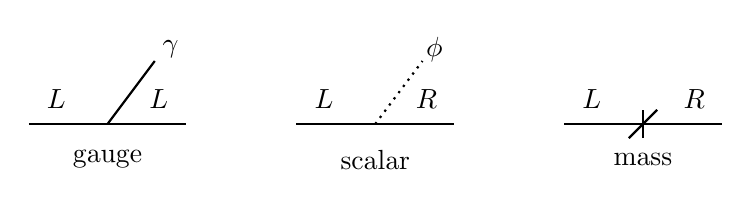
\begin{tikzpicture}[scale=1.0]
\draw[thick] (0,0)--(2,0);
\draw[thick] (1,0)--(1.6,0.8);
\node at (0.35,0.32) {$L$};
\node at (1.65,0.32) {$L$};
\node at (1.8,0.95) {$\gamma$};
\node at (1,-0.45) {gauge};

\draw[thick] (3.4,0)--(5.4,0);
\draw[dotted,thick] (4.4,0)--(5.0,0.8);
\node at (3.75,0.32) {$L$};
\node at (5.05,0.32) {$R$};
\node at (5.15,0.95) {$\phi$};
\node at (4.4,-0.45) {scalar};

\draw[thick] (6.8,0)--(8.8,0);
\draw[thick] (7.8,-0.18)--(7.8,0.18);
\draw[thick] (7.62,-0.18)--(7.98,0.18);
\node at (7.15,0.32) {$L$};
\node at (8.45,0.32) {$R$};
\node at (7.8,-0.45) {mass};
\end{tikzpicture}
\caption{Schematic chirality mnemonics: gauge emission preserves chirality, while scalar couplings and mass insertions flip it.}
\end{figure}

Now suppose the electron starts massless. Can photon emission and reabsorption generate a mass? No, because every gauge interaction preserves chirality, so no chain of such vertices can turn a left-chiral state into a right-chiral one. Can scalar emission and reabsorption generate a mass from zero? Again no, because emission and reabsorption require an even number of scalar vertices, hence an even number of chirality flips, which returns us to the original chirality instead of producing the \(L\leftrightarrow R\) transition characteristic of a mass term.

A nonzero correction appears only when a mass insertion is already present somewhere in the diagram. Then the correction is proportional to the original mass. The lecture summarizes this schematically as
\begin{equation}
m_e=m_0+O(e^2m_0)+O(e^4m_0)+\cdots.
\end{equation}
So if the starting fermion mass is zero, it stays zero; if it is small, it stays small. That is a very different situation from the scalar case, where large additive corrections appear regardless of whether one started massless.

\begin{remark}
The spoken lecture slides at moments between chirality and helicity language. For the mathematical statement here, chirality is the safer notion; in the relativistic limit the two coincide closely enough for the lecture's intuition to remain useful.
\end{remark}

Gauge bosons behave similarly in the sense relevant here: if they start massless, they remain massless to all orders. Hence the Standard Model's really serious fine-tuning problem is concentrated in the Higgs sector.

\subsection{Question \& Answer}

\paragraph{Question.} Why doesn't the electron have the same fine-tuning problem?

\paragraph{Answer.} Because its mass is protected against additive renormalization. Starting from \(m_0=0\), neither gauge-boson emission nor scalar emission-and-reabsorption can generate a chirality-flipping two-point term. Any correction to the electron mass must already contain one explicit mass insertion, and is therefore proportional to \(m_0\) itself. A small fermion mass may still be unexplained, but it is not produced by canceling huge ultraviolet contributions against one another.

\section{Vacuum Energy and the Supersymmetry Outlook}

The lecture closes by widening the discussion. There is another quantity that gets renormalized: the energy of the vacuum. In ordinary nongravitational physics, vacuum energy looks unimportant because only energy differences matter. We do not care about the absolute value of the vacuum energy so long as adding a particle adds the correct extra amount of energy. But if gravity is included, the vacuum itself gravitates, so its energy density becomes physically important.

In \(\phi^4\) theory a vacuum-to-vacuum diagram has no external particles at all. A short-distance estimate gives one factor of \(\lambda\) and two short propagators, hence
\begin{equation}
\delta\rho_{\mathrm{vac}}\sim \frac{\lambda}{\delta^4}.
\end{equation}
More complicated diagrams typically share the same qualitative \(\delta^{-4}\) behavior. Thus vacuum energy is also violently sensitive to short-distance physics.

The lecture's conclusion is therefore that there are at least two severe fine-tuning problems: the Higgs mass and the vacuum energy. Supersymmetry is introduced as a possible response to the first of these, not to the second. It may help prevent the Higgs mass from being driven to enormous values by renormalization, but it is not presented here as a solution to the cosmological-constant problem.

\subsection{Question \& Answer}

\paragraph{Question.} Does the fine-tuning depend on the arbitrary cutoff \(\delta\)?

\paragraph{Answer.} The contribution certainly depends on how far down in distance we trust the theory. But that is not an empty arbitrariness. We choose \(\delta\) to be the shortest scale at which we still believe the present quantum field theory makes sense. Then the accumulated contribution from all scales above that point is already there and must be accounted for. In that sense the estimate is a lower bound on how bad the problem is. If the theory continues to still shorter distances, the scalar fine-tuning can only become worse. The lecture mentions, as a plausible conservative benchmark, scales as small as unification, around \(10^{16}\,\mathrm{GeV}\), with the Planck scale making the tension still sharper.

Two late clarifications in the lecture are worth preserving. First, a scalar particle is simply a spin-zero particle; the Higgs is the central example here. Gauge bosons, by contrast, are spin-one particles. Second, although the simplest fermion and boson vacuum diagrams can come with opposite signs, they do not cancel automatically. Cancellation requires a delicate matching of masses and couplings. Supersymmetry is precisely the sort of structure that attempts to impose that matching, which is why it enters the story naturally at the end of this lecture.

\section{Summary}

The lecture begins by teaching us how to think about renormalization before it asks us to calculate anything. We first eliminate fast electrons in a molecule and replace them by an effective potential. Then we translate the same logic to quantum field theory, where short-distance modes renormalize the parameters in the Lagrangian. For scalar fields the mass term receives large additive corrections, and this becomes the Higgs hierarchy problem once the cutoff is taken seriously. Fermions and gauge bosons are better behaved because their masses are protected when they start from zero. The lecture then widens once more to vacuum energy, whose renormalization becomes a second fine-tuning problem when gravity is allowed to care about the vacuum. Supersymmetry appears at the end not as a finished theory, but as the natural next question.